\documentclass[english,seminar]{lecture}

\usepackage{float}
\usepackage{tikz}
\usetikzlibrary{patterns}
\usepackage{wrapfig}
\usepackage{amsmath}
\newcommand{\diff}{\,\textrm{d}}

\title{Spacetime}
\subtitle{Special and General Relativity}
%\shorttitle{}
%\ccode{}
\subject{Physics}
\speaker{V.H. Belvadi}
\spemail{vh@belvadi.com}
%\author{}
%\email{}
%\flag{}
%\season{}
%\date{}{}{}
%\dateend{}{}{}
%\conference{}
%\place{}
%\attn{}
\morelink{vhbelvadi.com/teaching}

\begin{document}
\section{Minowski spacetime}\label{sec:minkowskispacetime}
In relativity we often talk about `events'. This is a broad term meaning any phenomenon or object under observation, such as a lightning strike, a ball rolling on the floor, a vehicle crossing a certain point in space, clocks ticking, you reading these notes now etc. It is essentially anything to which we can assign a point in space and in time.

In speaking of time, simultaneity is a key concept. Think of a beam of light leaving a point A when your watch ticks $t_A$ and reaching a point B at $t_B$ and returning to point A at $t_A'$. There is \textbf{simultaneity} if $t_B - t_A = t_A' - t_B$ i.e. the initial and final time periods match exactly. Given $c$ is the speed limit of the universe (the only sound explanation we can think of to the Michaelson--Morley experiment that failed to detect a hypothesised `\ae ther` in space) we define $c$ as
\[
{2AB \over t_A' - t_A} = c
\]
There is another way to look at this: if a light wave starts at some origin point in spacetime and travels to some $(x,y,z)$ and it takes time $t$ to undergo this displacement we can write the following equation knowing $c$ is the velocity at which light travels:
\[
x^2 + y^2 + z^2 = c^2t^2
\]
which, strictly speaking, is obtained from spatial and temporal differences:
\[
(x_2-x_1)^2 + (y_2-y_1)^2 + (z_2-z_1)^2 = c^2 (t_2-t_1)^2
\]
Observe that the right-hand side of this equation is essentially the distance formula in Cartesian space. A single unit of length $\diff s$ can then be expressed in terms of $\diff x$, $\diff y$, $\diff z$ and $-c\diff t$. We will now formalise this idea.

A vector $\mathbf{A}$ in frame $S$ is defined in terms of four components as \[\mathbf{A} \xrightarrow{S} (t,x,y,z) \quad\Longleftrightarrow\quad \mathbf{A} \xrightarrow{S} {x^\mu}\]where the components refer to time and space in that order. We can just as well represent them as space first followed by time but we will retain the above ordering throughout this course for uniformity. For simplicity we will favour the equivalent notation given on the right\footnote{If you are familiar with tensors you will recognise such a subscript notation as the one used here; if not, just remember that when we write $x^2$ for $\mu = 2$ we mean $2$ as a subscript, not as a power.}. The greek alphabet used in the index will be assumed to imply $n$ co-ordinates, in this case $n=4$ counting from zero, i.e. $\mu = 0$ to $3$ with $x^0 = t$, $x^1=x$, $x^2=y$ and $x^3 = z$. Keep in mind that these are indices, not powers. If you use the $(x,y,z,t)$ ordering $n$ will go from $1$ to $4$ with $x^4 = t$. In any case the indices $1$ to $3$ are, by convention, retained for spatial co-ordinates like $x$, $y$ and $z$. Keep in mind that using bold letters becomes redundant when referring to tensorial forms, e.g. $U^\mu$ is a vector.

As an example let us see how this notation can eventually help us simplify the familiar Lorentz transformations. Say we want to displace ourselves over $\mathbf{s}$ in some coordinate system (which we will name in a moment). The magnitude of our displacement would be given by $(\Delta s)^2 = (\Delta x)^2 + (\Delta y)^2 + (\Delta z)^2 = c^2 (\Delta t)^2$ or, more conveniently,\margintext{For more discussion on this see \cite{chappell} which also discusses the action integral in this context.}
\begin{align}
	(\Delta s)^2 &= -(c\Delta t)^2 + (\Delta x)^2 + (\Delta y)^2 + (\Delta z)^2 \label{eq:s2} \\
	\textrm{(equivalently)} \qquad (\Delta s)^2 &= -(\Delta x^0)^2 + (\Delta x^1)^2 + (\Delta x^2)^2 + (\Delta x^3)^2 \nonumber
\end{align}%
which is the spacetime interval between two points in space whose each $x^\mu$ coordinate is separated by $\Delta x^\mu$. You may at first think this is simply a modification of the usual distance formula between coordinate pairs. However, keep in mind that $\Delta s$ is \textit{not} physical distance anymore in four-dimensional spacetime but simply a mathematical quantity known as the \textbf{spacetime invariant}.

In other words we have a system of co-ordinates involving temporal and spatial components that look like\margintext{Observe this method of breaking down the four $\mu$ indices into a zero and three $i$ indices. We will use this a lot going forwards.} $x^\mu \equiv (x^0, x^i)$  This lets us define a set of co-ordinates, or a system, which we call \textbf{Minkowski spacetime} with $x^0 = ct$, $x^1 = x$, $x^2 = y$ and $x^3 = z$. Again, these are indices, not exponents---context clarifies that. Let us now also quickly clarify our notations: we will use greek alphabets to refer to Minkowski spacetime and latin alphabets to refer to `normal', three-dimensional co-ordinates, e.g. $x^\mu \equiv (x^0, x^1, x^2, x^3)$ while, as usual, $x^i \equiv (x^1, x^2, x^3)$.

Finally, consider, for simplicity, the scale $c=1$ with co-ordinates $(t,x,y,z)$, and use latin alphabets to refer to `normal' three-dimensional space with co-ordinates $(x,y,z)$. The scale $c=1$ means $3\times 10^8$\,ms$^{-1}$ is equal to $1$ or, equivalently, $1\,\textrm{s} = 3\times 10^8$\,m. Another way to think of this is that scaling $c=1$ lets us express everything else in units of energy, e.g. $E^2 = p^2c^2 + m_0^2c^4$ (a formula you will come across later) in \textbf{natural units} (where $\hbar = c = k_B = 1$) gives us mass and momentum in units of energy.\footnote{`Natural system of units in general relativity' by A.L. Myers (see tables 1 and 3) available at \url{seas.upenn.edu/~amyers/NaturalUnits.pdf} gives a good explanation of natural units.} This does alter the dimensions of certain quantities so when we need an absolute final result we simply set the dimensions right by multiplying by $c$ as appropriate. There is also another system of units called `Geometrised units', where $c=G=1$, that you will come across in General Relativity.

%
%
%
%
%
%
%

\section{Lorentz transformations}\label{sec:lorentzTransformations}

Our next step is to try to write down the familiar Lorentz transformations. We will try to keep things simple. Let us start by making eq. \eqref{eq:s2} compact using matrices. Notice that in writing down our co-ordinates $(t,x,y,z)$ we did not carry over the one negative and three positive signs in that equation. That is because these signs are best defined as part of a \textbf{metric tensor} with components $\eta_{\mu\nu}$ as follows
\begin{equation}
\eta_{\mu\nu} =
\begin{pmatrix}
	-1 & 0 & 0 & 0 \\
	0 & 1 & 0 & 0 \\
	0 & 0 & 1 & 0 \\
	0 & 0 & 0 & 1
\end{pmatrix} \label{eq:minkowskiTensor}
\end{equation}%
then eq. \eqref{eq:s2} is nothing but
\begin{equation}
	\Delta s^2 = \eta_{\mu\nu}\Delta x^{\mu}\Delta x^{\nu} \label{eq:smatrix}
\end{equation}%
where the summation convention\footnote{According to this convention the right-hand side of eq. \eqref{eq:smatrix} is $\eta_{00}\Delta x^0\Delta x^0 + \eta_{01}\Delta x^0\Delta x^1 + \ldots + \eta_{21}\Delta x^2\Delta x^1 + \eta_{22}\Delta x^2\Delta x^2 + \ldots + \eta_{33}\Delta x^3\Delta x^3$, with nine terms in all.} is used. To wit, the summation convention tells us that \textit{when an index is repeated as both a subscript and a superscript it must be summed over an appropriate range}.

The signs of eq. \eqref{eq:minkowskiTensor} are often written down as $(-,+,+,+)$. This is known as the \textbf{metric signature}. This is often also denoted by $(1,3)$ for obvious reasons and, less helpfully, by its trace $2$.

It is worth pausing here to take note of a key alternative route to these equations. Had we written $(\Delta s)^2 = (\Delta x)^2 + (\Delta y)^2 + (\Delta z)^2 = c^2 (\Delta t)^2$ in mostly negative terms as $(\Delta s)^2 = - (\Delta x)^2 - (\Delta y)^2 - (\Delta z)^2 + c^2 (\Delta t)^2$ we would have ended up with a different form of $\eta$ where the positive and negative signs would have switched to give the signature $(-,+,+,+)$ or trace $-2$. While the choice between these $(1,3)$ signatures is personal rather than mathematical, most relativists prefer the former convention because it keeps space familiarly positive, requiring us to deal with just one negative term while particle physicists prefer the latter convention as it makes some of their equations, particularly the important $p^\mu p_\mu = m_0^2$, positive and more convenient.

Back to relativity: We now need to find a convenient transformation between reference frames where eq. \eqref{eq:smatrix} holds. We know transformations to be a procedure that alters our system while keeping a particular factor universally consistent; the `particular factor' in our case is the spacetime interval. That is to say, we need a transformation that keeps $\Delta s^2$ unchanged.

Generally speaking a simple transformation can be something as straightforward as addition: to take $x^\mu \rightarrow x^{\mu '}$ we can define some $\alpha^\mu$ that satisfies $x^{\mu '} = x^\mu + \alpha^\mu$. But we can go a step further and generalise this with multiplication too---after all addition is contained within multiplication. So, say we have a matrix $\Lambda$ that satisfies
\begin{equation}
x^{\mu '} = \Lambda^{\mu '}_\nu x^\nu \quad \textrm{or simply} \quad x' = \Lambda x \label{eq:LambdaTransformation}
\end{equation}%
We can then require that
\begin{align}
	(\Delta s)^2 = \eta_{\mu\nu} \Delta x^{\mu } \Delta x^{\nu }
		&= \eta_{\mu'\nu'} \Delta x^{\mu '} \Delta x^{\nu '} \;\;\;\textrm{(Invariance)} \nonumber\\
		&= \left( \Delta x^{\mu '} \right)^T \eta_{\mu'\nu'} \left( \Delta x^{\nu '} \right) \nonumber\\
		&= \left( \Delta x^\nu \right)^T \Lambda^{\mu'^T}_\nu \eta_{\mu'\nu'} \Lambda^{\nu'}_\mu \left( \Delta x^\mu \right) \nonumber\\
		&= \eta_{\mu'\nu'} \Lambda^{\mu'}_\nu \Lambda^{\nu'}_\mu \Delta x^\mu \Delta x^\nu \nonumber\\
\textrm{(generalising indices)} \quad \therefore \eta_{\sigma\rho} &= \Lambda^{\mu'}_\sigma \Lambda^{\nu'}_\rho \eta_{\mu'\nu'} \label{eq:lorentzCondition}
\end{align}%
What this tells us is that if we find appropriate $\Lambda$ matrices our metric tensors $\eta_{\mu\nu}$ and $\eta_{\mu '\nu '}$ transform as above then we have our transformation. Keep in mind that we could have used alternate, simpler indices like, say, $\alpha$ and $\beta$ instead of $\mu '$ and $\nu '$ but we retained the latter because the prime serves to remind us what terms the transformation is affecting and that it is across frames\footnote{We will clarify some of the physical ideas behind our discussion as we go on, so we will focus on establishing some results and properly developing our mathematical language right now.}.

\\\runin{At this point} we shall introduce two more terms: \textbf{proper measures} and \textbf{coordinate measures}. Suppose some event takes place along a path and an observer outside is watching this, the proper time is the time measured by a clock traveling along the path, or by the event itself, while the coordinate time is that measured by the external observer. Similarly, proper space and co-ordinate space are for lengths.

All this presents an interesting consequence for the time period involved. For our spacetime interval, which we shall now call $\diff s^2$, given by eq. \eqref{eq:s2}, and from the general transformation defined by eq. \eqref{eq:LambdaTransformation} we have a time interval defined by $\diff \tau^2 = \diff t^2 - \diff x^2 \equiv -\eta_{\mu\nu}\diff x^\mu \diff x^\nu$ which works because the second term on the right-hand side also has temporal dimensions in natural units, i.e. when $c=1$. Our exercise now is to proceed by using the same logic as we did while attempting to arrive at eq. \eqref{eq:lorentzCondition} above.\footnote{Note that although eq. \eqref{eq:tau} seems to imply the relation $\diff s^2 = - \diff \tau^2$ the exact relation is $\diff s^2 = -c^2 \diff \tau^2$ but $c^2$ vanishes in natural units. This, in fact, is how we got $\diff \tau^2 = \diff t^2 - \diff x^2$.}
\begin{align}
	\diff \tau^2 &= \diff t^2 - \diff x^2 \label{eq:tau} \\
				&\equiv -\eta_{\mu\nu}\diff x^\mu \diff x^\nu \nonumber\\
				&= -\eta_{\mu '\nu '} \Lambda^{\mu '}_{\nu} \Lambda^{\nu '}_{\mu} \diff x^{\mu} \diff x^{\nu} \nonumber\\
				&= -\eta_{\mu ' \nu '} \diff x^{\mu '} \diff x^{\nu '} \nonumber\\
				&\equiv \diff t'^2 - \diff x'^2 \nonumber\\
\implies \diff \tau^2 &= \diff \tau '^{2} \label{eq:tau=tauPrime}
\end{align}%
The $\Lambda$ transformation\footnote{Also read about the \textit{inhomogeneous Lorentz group}, a set of Lorentz transformations that obey eq. \eqref{eq:LambdaTransformation}.  We also call this the Poincar\'{e} group.} came to our aid once again. Equation \eqref{eq:tau=tauPrime} is a key result in special relativity: \textit{proper time is invariant under a Lorentz transformation}. This result is important historically too: for a beam of light, when you measure the velocity of light as $\diff x/\diff t = c = 1$ in one frame (and $\diff t/\diff t = 1$ as usual), eq. \eqref{eq:tau=tauPrime} assures us that $\diff \tau^2 = 1 - 1 = 0$ is equal to $\diff \tau'^2$ which means, in another frame, $\diff x'/\diff t' = c = 1$ as well. In other words, we have shown that \textit{the speed of light in both frames is a constant}. At this juncture we note that not only is proper time an invariant like the spacetime interval (i.e. $\diff S^2 = \diff S'^2$), it is also proportional to the spacetime interval:
\begin{align}
	\diff \tau \propto \diff S \label{eq:s-tau-proportionality}
\end{align}%
%
\\\runin{Talking for too long} in generalised terms of $\Lambda$ may have made things hazier than intended, so let us try to give a specific form for $\Lambda$. The result that we will finally arrive at will probably not surprise you at all; the steps themselves are few and simple.

First, we can rewrite eq. \eqref{eq:tau} as $\diff \tau^2 = \diff t^2 \left(1 - v^2\right)$ but remember that we are using natural units so we have used $c^2=1$ here. For exactness we can bring $c$ back, which means removing $c^2\diff t^2$ in common from the right-hand side of eq. \eqref{eq:tau}. Doing this gives us $\diff \tau^2 = \diff t^2 \left(1 - v^2/c^2\right)$ which is an expression you would have previously encountered. The ratio $v/c$ is conventionally represented by $\beta$ and we will use this convention here too. In fact, as an exercise, try doing the same thing with eq. \eqref{eq:s2} and you will once again obtain the $\left(1-\beta^2\right)$ factor as in this equation.

The Lorentz transformation equation can, in fact, be written in a compact manner like eq. \eqref{eq:smatrix}. We already know that, for frames moving along the x-axis with a relative velocity of $v$, at some time $t$, the relation $x' = x - vt$ is valid. Likewise $t' = t - vx$ must also be valid\footnote{All of this is under the assumption that there is no motion along the $y$ and $z$ directions for simplicity without sacrificing generality. Also, $c=1$ but perhaps we should stop explicitly reminding ourselves of that now.}. We realise this equivalence is not accurate, though, so we bring in some correction factors: let us rewrite these equations as \[x' = \gamma (x - vt) \qquad \textrm{and} \qquad t' = \gamma (t - vx)\]
To find $\gamma$ we need to bring in some sort of relation between $x'$ and $t'$ but we do not have to look far for that\footnote{The reason we chose the same $\gamma$ for $x'$ and $t'$ both, rather than two different correction factors, will be clarified in \S\ref{sec:spacetime-diagrams} where we show that $x'$ and $t'$ vary similarly. For now take this for granted.}. The spacetime invariance must hold in both frames (that is why it is an \textit{invariance}) so eq. \eqref{eq:s2} readily gives us \[-\Delta t'^2 + \Delta x'^2 = -\Delta t^2 + \Delta x^2\] ignoring the $y$ and $z$ directions once again. Consequently we get\footnote{These steps are left as an exercise.} \[\gamma = \pm{1\over\sqrt{1-v^2}}\] which is the Lorentz factor we are probably already aware of. We normally call this $\gamma$ and have used natural units here. To complete our discussion we write down the full set of Lorentz transformations:%
\begin{subequations} \label{eq:lorentzTransformations}
	\begin{align}
		t' &= {t-vx\over\sqrt{1-v^2}} \label{eq:lorentz-t}\\
		x' &= {x-vt\over\sqrt{1-v^2}} \label{eq:lorentz-x}
	\end{align}%
\end{subequations}%
Note that we have left out the trivial $y' = y$ and $z' = z$ cases\footnote{Also, eq. \eqref{eq:lorentz-t} and \eqref{eq:lorentz-x} in standard units carry the denominator $\left( 1 - (v^2 / c^2) \right)^{-1/2}$ or, equivalently, the factor $\gamma$ so that $t' = \gamma (t-vx)$ and $x' = \gamma (x-vt)$, in a form you know more intimately.}.

However, why did we do all this? We find that eq. \eqref{eq:lorentzTransformations} can be put into a compact matrix form too, somewhat like eq. \eqref{eq:lorentzCondition}. Rather than $\eta_{\mu\nu}$ we now have a $\Lambda$ matrix that looks like
\[
\Lambda = 
\begin{pmatrix}
	\gamma & -v\gamma & 0 & 0 \hspace*{0.15cm}\\
	-v\gamma & \gamma & 0 & 0 \hspace*{0.15cm}\\
	0 & 0 & 1 & 0 \hspace*{0.15cm}\\
	0 & 0 & 0 & 1 \hspace*{0.15cm}\\
\end{pmatrix}
\]
and forms the beautiful \textbf{Lorentz transformation} equation:
\begin{equation}
	x^{\mu '} = \Lambda^{\mu '}_\nu x^\nu \label{eq:LorentzTransformationCompact}
\end{equation}%
This is exactly what we saw earlier as eq. \eqref{eq:LambdaTransformation} but we now know the meaning of $\Lambda$ and that $\Lambda^{\mu '}_\nu$ refers to the $\mu^{\textrm{th}}$ row and $\nu^{\textrm{th}}$ column of our $\Lambda$ matrix\footnote{To verify the $\Lambda$ matrix try substituting values for $\mu$ and $\nu$ into eq. \eqref{eq:LorentzTransformationCompact}, e.g.%
\begin{align*}
	x'^{1} &= \Lambda'^{1}_{0} x^{0} + \Lambda'^{1}_{1} x^{1} + \Lambda'^{1}_{2} x^{2} + \Lambda'^{1}_{3} x^{3} \\
\implies x' &= -v\gamma t + \gamma x + 0 + 0 \\
\therefore x' &= \gamma (x - vt)
\end{align*}%
which is the same as eq. \eqref{eq:lorentz-x}. Try plugging in $\mu = 0$ for eq. \eqref{eq:lorentz-t} next.
}.

%
%
%
%
%
%
%

\section{Spacetime diagrams}\label{sec:spacetime-diagrams}

All of the work we did so far and will do in the future, in relation to Special Relativity, must abide by two core ideas: first, the \textbf{principle of relativity} demands that the laws of physics be consistent in all frames of reference; second, Einstein capped this law with a speed limit showing the \textbf{universality of the speed of light}, i.e. the value of $c$ in a vacuum cannot be superseded without breaking causality\footnote{`Causality' is the idea that effects cannot precede cause, i.e. that the cause always comes first and the effect follows it. Look up any thought experiment on causality, e.g. a car appearing to swerve around an obstacle on an intersection before the obstacle itself appears, or a cup breaking to pieces before it falls etc.}.

\begin{wrapfigure}{l}{0.55\textwidth}
%\vspace*{-6.5ex}
%\begin{figure}
	\vspace*{1cm}
	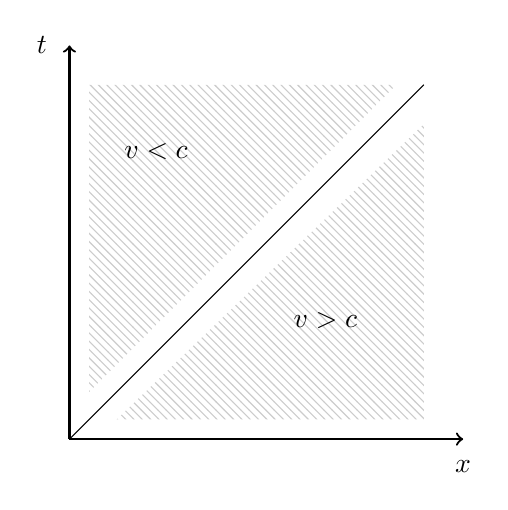
\begin{tikzpicture}
		\draw[thick,->] (0,0) -- (0,5);
		\draw[thick,->] (0,0) -- (5,0);
		\draw (0,0) -- (4.5,4.5);
		\fill[pattern=north west lines, pattern color=black!20!white,thin] (0.25,0.6) -- (4.15,4.5) -- (0.25,4.5);
		\node at (1.1,3.65) {$v<c$};
		\fill[pattern=north west lines, pattern color=black!20!white,thin] (0.6,0.25) -- (4.5,0.25) -- (4.5,4);
		\node at (3.25,1.5) {$v>c$};
		\node at (5,-0.35) {$x$};
		\node at (-0.35,5) {$t$};
	\end{tikzpicture}
	\caption{Basic spacetime diagram.}\label{fig:spacetime-diagram}
	\vspace*{1cm}
%\end{figure}
%\vspace*{-2.5ex}
\end{wrapfigure}

The best way to appreciate relativity geometrically is through spacetime diagrams. These are graphs of time against usually one dimension of space (conventionally $x$ due to \textbf{isotropy}, the valid assumption that there is nothing special about either the $x$ or the $y$ or the $z$ directions so we can pick any to represent all three). This also calls for a clarification of what the word `space' means. In relativity \textbf{space} is simply any continuous collection of points or co-ordinates; the key requirement here being continuity as opposed to discreteness.

On a graph of $t$ versus $x$ we know that the slope $\diff t/\diff x$ would give us the (reciprocal of) velocity. So what would the line $v = c = 1$ look like? It should naturally be a line of slope $1$, i.e. a line at precisely 45$^\circ$ on our spacetime diagram. This is shown in fig. \ref{fig:spacetime-diagram}. 

Recall from our definition of an event earlier that it can be any occurrence in space and time; that is, an \textbf{event} is any record of $(t,x,y,z)$ co-ordinates. On a spacetime diagram every point represents an event.

If you mark several such events, or points, for, say, a particle traveling in space, you end up with a line that describes the progression of the spacetime co-ordinates associated with the particle. We call such a line the \textbf{world line} of that particle. The world line of light is shown in fig. \ref{fig:spacetime-diagram} and is, as explained earlier, a line of 45$^\circ$ slope for $v=c=1$. In the region above this more time passes for a given distance, i.e. $v<c$, and in the region below this less time passes for a given distance, i.e. $v>c$.

This leads us to two further classifications. If an event lies in a region of our spacetime diagram where there is more space than time we say the event is \textbf{spacelike}. In such cases the spacetime interval\footnote{A quick reminder: the spacetime interval is $\diff s^2$ and not $\diff s$ itself.} $\diff s^2 < 0$ and our event lies in the $v > c$ region of a spacetime diagram (see fig. \ref{fig:spacetime-diagram}). Similarly, if an event lies in a region where there is more time than space and where, consequently, $\diff s^2 > 0$, we say the event is \textbf{timelike}. Such events lie in the $v < c$ region of a spacetime diagram (once again, consult fig. \ref{fig:spacetime-diagram}). Additionally, a \textbf{lightlike} event is one that lies on the $v = c$ line; it behaves `like light'. We also sometimes call such spacetime intervals \textbf{null} in reference to `null' or nonexistent quantities because $v=c$ is not achievable except by photons.

\begin{figure}[H]
\vspace*{0.25cm}
\centering
	\begin{tikzpicture}
		\draw[thick,<->] (0,-4) -- (0,4.5);
		\draw[thick,<->] (-5,0) -- (5,0);
		\draw (5,4) -- (-3,-3);
		\draw (-1,4) -- (4,-2);
		\draw[dashed] (-3,3) -- (2.25,-3);
		\draw[dashed] (2,3.5) -- (-4,-2);
		
		\node[circle,inner sep=1pt,fill=black,label=left:{B}] at (-1.025,0.725) {};
		\node[circle,inner sep=1pt,fill=black,label=right:{A}] at (1.525,0.965) {};
		\node at (5,-0.35) {$x$};
		\node at (-0.35,4.5) {$t$};
		
		\node at (5,4.35) {$L$};
		\node at (-1.25,4.25) {$M$};
		\node at (4.25,-2.25) {$N$};
		\node at (-3.2,-3.2) {$O$};
		\node at (0.6,2.6) {$P$};
		\node at (-3.25,3.25) {$W$};
		\node at (-4.25,-2.25) {$U$};
		\node at (2.5,-3.25) {$Q$};
		\node at (2.25,3.75) {$R$};
		\node at (-0.4,-0.4) {$K$};
	\end{tikzpicture}
	\caption{Light cones for events A (solid) and B (dashed). The lines OL, MN, WQ and UR denote $v=c=1$ and are the world lines of photons; they are said to be \textit{lightlike}. The region inside a light cone is \textit{timelike} and the region outside is \textit{spacelike}.}\label{fig:light-cones}
\end{figure}

In many ways a spacetime diagram is just like a position--time graph\footnote{The brief introduction to spacetime diagrams provided in this section is sufficient for our purposes but it is not exhaustive. You can go over \S1.5 in \cite{schutz} for several more interesting discussions.}: constant velocity is represented by a straight-line while acceleration is represented by a curved line. The only point to remember is that there is a speed limit in spacetime diagrams that results in the world line of light, or of photons in a vacuum, being equidistant from the $x$ and $t$ axes throughout the graph.

Let us now expand the world line of light in all possible directions of space. This is shown in fig. \ref{fig:light-cones}. You may wonder, initially, what the lines going backwards in time mean, but remember that this is not a position--time graph of the progression of a particle with time rather a spacetime diagram that simply associates with each event four co-ordinates of Minkowski spacetime. Say we have arbitrary events A and B. The photon world lines from those events are as shown in the figure above. We are aware from our previous discussion that the region outside the `cones' formed by MAL and OAN for event A (and WBR and UBQ for event B) are forbidden since $v>c$ here. In other words, if you were at A or at B, only something in the region of your \textbf{future light cone} will happen next; likewise only something in the region of your \textbf{past light cone} could have happened before this point in time. In the region of MPR the events A and B may interact; in the past they may only have interacted beyond the OKQ overlap of their past light cones. It is physically impossible for them to gain any knowledge of events in their \textit{spacelike} region as they now stand.

\begin{wrapfigure}{l}{0.55\textwidth}
%\vspace*{-6.5ex}
%\begin{figure}
%	\vspace*{1cm}
	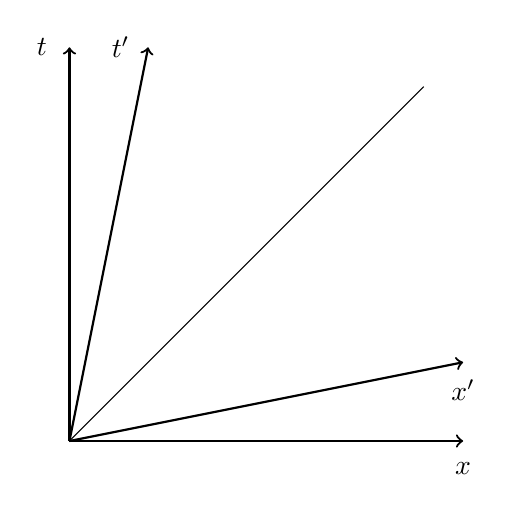
\begin{tikzpicture}
		\draw[thick,->] (0,0) -- (0,5);
		\draw[thick,->] (0,0) -- (1,5);
		\draw[thick,->] (0,0) -- (5,0);
		\draw[thick,->] (0,0) -- (5,1);
		\draw (0,0) -- (4.5,4.5);
		\node at (5,-0.35) {$x$};
		\node at (-0.35,5) {$t$};
		\node at (5,0.65) {$x'$};
		\node at (0.65,5) {$t'$};
	\end{tikzpicture}
	\caption{Basic spacetime diagram.}\label{fig:spacetime-two-frames}
%\end{figure}
%\vspace*{-2.5ex}
\end{wrapfigure}

\\\runin{The usefulness of} spacetime diagrams becomes clear when we consider how they help us relate multiple frames of reference. Consider a primed and an unprimed frame. Say we were to plot the positions of two sets of clocks $A$ and $B$. If they were placed 10\,m apart while relatively at rest, we have plots that are simple enough. But if one of them, say the set $B$, starts to move on a conveyer belt at $v = 0.87c$ antiparallel to the other, $A$ would notice \textbf{length contraction} in $B$ so that to appear spaced 10\,m apart the $B$  clocks would have to be placed $L_B = L_A/\gamma \approx 20$\,m apart. Conversely, from the $B$ perspective, the clocks of set $A$ would have to be placed $L_A = L_B \gamma \approx 5$\,m apart.

Plotting these world lines on two frames of reference (one for the $x-t$ system and another for the $x'-t'$ system) we would notice that the lines joining the intersections where corresponding clocks would be simultaneous i.e. clock $A_1$ simultaneous with $B_1$, $A_2$ with $B_2$ etc., known as the \textbf{lines of simultaneity}, would correspond with their respective x-axes. This is immediately apparent in case of the $x-t$ system for $A$, so finding the line of simultaneity in the $x'-t'$ diagram for $B$ would give us its x-axis. These results give us a combined figure like in fig. \ref{fig:spacetime-two-frames} which represents two frames of reference in a single spacetime diagram. We could also represent the $x'-t'$ frame as perpendicular and choose to make $x-t$ obtuse.

Using fig. \ref{fig:spacetime-two-frames} as our standard diagram, observe that any point on the $t'$ axis when transformed onto the $t$ axis by drawing a line from $t'$ to $t$ parallel to the $x'$ line would put the equivalent point on $t$ closer to the origin than the original point on $t$ axis, drawn similarly but using a line parallel to $x$ this time. In other words, for a point on the $t'$ axis we can draw two lines to the $t$ axis, one parallel to $x'$ and one parallel to $x$, which would represent the value of $t'$ on $t$ and the value of $t$ on itself respectively. This would show us that $t > t'$ i.e. that frame $A$ of the $x-t$ system would notice longer times passing between two events than frame $B$ of the $x'-t'$ system, a demonstration of the phenomenon we know as \textbf{time dilation}.

Curiosity leads us to see what would happen if we kept increasing $v$, even as continuous acceleration and not just absolute skips: we would keep going closer to, but never fully overlap with, the $v=c$ line. We measure such accelerations hypothetically by putting ourselves on \textbf{instantaneously co-moving frames} or ICF for short which effectively allows us to write down the proper measures of that frame with which we are instantaneously co-moving.

\begin{thebibliography}{99}
	\bibitem{chappell}
	Chappell JM, Hartnett JG, Iannella N, Iqbal A, and Abbott D. Exploring the origin of Minkowski spacetime. \href{https://arxiv.org/abs/1501.04857}{\ttfamily arXiv:1501.04857}
	\bibitem{schutz}
	Schutz B. A first course in general relativity. Cambridge University Press. 2nd edition, 2009.
	\bibitem{einstein}
	Einstein A. On the electrodynamics of moving bodies. Translated from the original 1905 paper in `The Principle of Relativity'. Methuen and Company, Ltd., 1923.
\end{thebibliography}

\end{document}